\subsection{Dataflow analysis}
\begin{frame}
	\frametitlesubs

	\begin{itemize}
		\item Control Flow Graph (CFG)
			\begin{itemize}
				\item プログラムの流れをグラフで表したもの
			\end{itemize}
		\item Define-Use / Use-Define Chain (DU/UD Chain)
			\begin{itemize}
				\item 変数の定義、使用を調べる
				\item 役割としてはSSA、A正規形
			\end{itemize}
	\end{itemize}
\end{frame}

\subsubsection{Control Flow Graph}
\begin{frame}[fragile]
\frametitlesubs
\begin{minipage}{.23\textwidth}
	\scriptsize
	\begin{lstlisting}[language={[5.3]lua},numbers=none]
local b = true

if b then
	print("hello")
else
	print"world"
end
\end{lstlisting}

\pause
\vspace{-2\zw}
\begin{center}
	\normalsize
\noindent$\Downarrow$
\end{center}
\vspace{-2\zw}
\begin{lstlisting}[numbers=none]
LOADBOOL      0   1    0
TEST          0   0 
JMP           0   4 
GETTABUP      1   0   -1
LOADK         2   1 
CALL          1   2    1
JMP           0   3 
GETTABUP      1   0   -1
LOADK         2   2 
CALL          1   2    1
RETURN        0   1 
\end{lstlisting}
\end{minipage}\pause
\begin{minipage}{.06\textwidth}
\begin{flushright}
	\ $\Rightarrow$
\end{flushright}
\end{minipage}
\begin{minipage}{.56\textwidth}
	\begin{figure}[h]
	\centering
	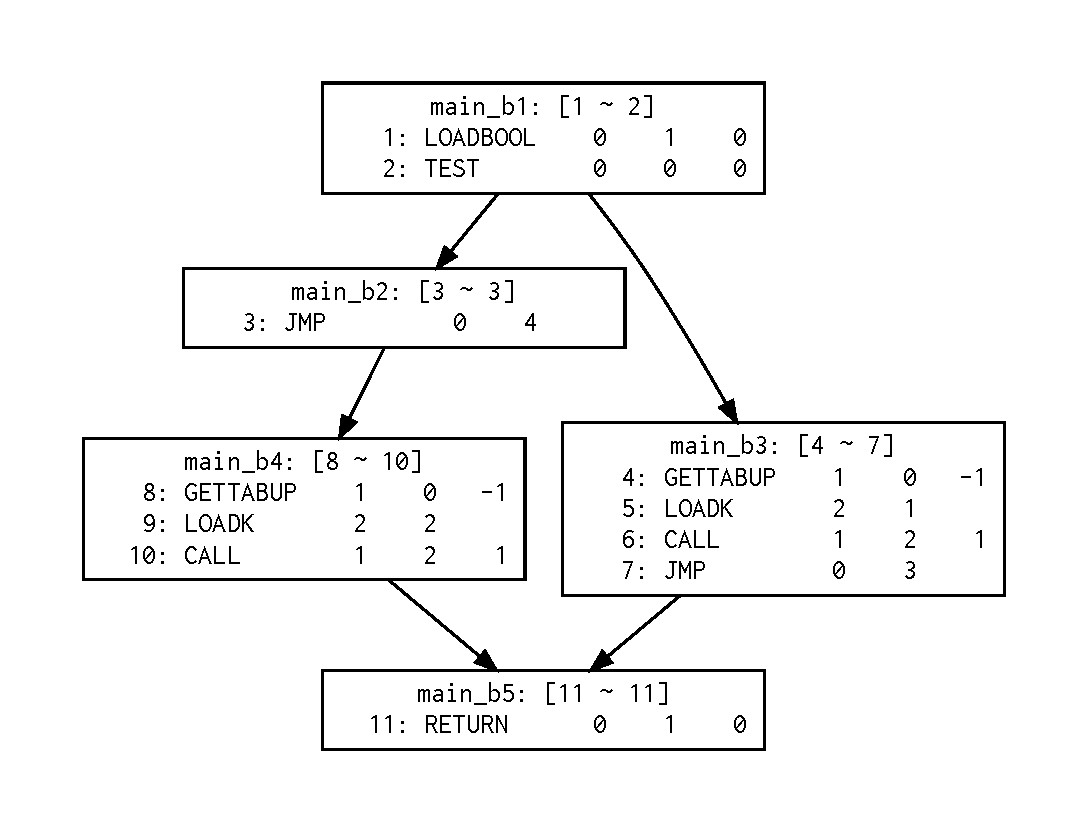
\includegraphics[width=1.3\textwidth]{img/cfg.pdf}
	\end{figure}
\end{minipage}
\end{frame}

